% Discuter les résultats, sources d'incertitudes, ...
Commençons par discuter les résultats dans leur globalité avant de discuter les multiples sources d'erreurs et d’imprécisions. Il faut tout d'abord noter que les filtres fonctionnent globalement comme espéré. Néanmoins, utiliser les mesures faites sur ceux-ci ne sont pas très précis pour la mesure de leur composant, et il serait donc à privilégier des montages dédiés à la mesure de l'inductance et de la capacité. De plus, sur les mesures correctes, tout cela permet de confirmer les bonnes prédictions du modèle $RL$ et $RC$ dans son ensemble.\\ \\
De manière plus détaillée, le filtre "passe-bas" par la \textit{self} donne de bon résultat. Malgré l'oubli de la mesure de la tension d'entrée, on peut l'estimer par les valeurs plateaux de la tension à la résistance, soit pour $R=5 \ [\Omega]$ autour de $5.65 \ [V]$ et la courbe de tendance retrouve un peu plus haut ($5.969 \ [V]$), ce qui est raisonnable. Il en est presque de même pour celle de $50 \ [\Omega]$ (estimé $\sim 8.32 \ [V]$ / tendance $\sim 8.310 \ [V]$). La différence entre la tension pour les deux résistances s'explique car il a fallu l'augmenter afin de mieux voir les différentes courbes sur l'oscillateur.\\
Pour le déphasage, on observe néanmoins un écart relativement élevé. Cela peut s'expliquer par le protocole de mesure de l'intervalle temporel se faisant à la main avec les curseurs de l'oscilloscope. On aurait par exemple pu être plus précis en important les courbe sur un ordinateur et faisant un script pour mesurer l'intervalle de temps. Cette impact est clairement visible sur les valeurs de l'inductance qui dépendent de la mesure du déphasage, lui même linéairement de l'écart temporel. Et sur ce calcul de l’inductance, nous observons des écarts non-négligeables, que ce soit avec la valeur issue des spécifications ($\sim 33 \ [\%]$ d'écart avec la moyenne pour $R=5 \ [\Omega]$ et $\sim 15 \ [\%]$ pour $R=50 \ [\Omega]$), mais également entre les mesures (l'écart-type représente $\sim 40 \ [\%]$ de la moyenne pour $R=5 \ [\Omega]$ et $\sim 22 \ [\%]$ pour $R=50 \ [\Omega]$). Au premier ordre, on peut considérer la tangente comme linéaire et donc estimer une erreur similaire sur l'intervalle de temps.\\
On peut finalement émettre l'hypothèse que la fréquence de coupure est linéairement dépendant de la résistance (car pour $5 \ [\Omega]$, $f_c \sim 10^3$ et pour $50 \ [\Omega]$, $f_c \sim 10^4$) mais cela devrait être confirmé par une autre expérience ou un travail mathématique qui ne sera pas fait ici (quoique intuitivement, $I$ dépend "quasi-linéairement" - dû au carré puis la racine qui modifie légèrement cette dépendance, mais c'est négligeable - de $\frac{1}{R}$ ce qui décale la fréquence de coupure selon $R$). Selon des hypothèse similaire, on peut aussi conjecturer que c'est dépendant de $\frac{1}{U_{in}}$ (pour $U_{in} \sim 5 \ [V]$, le chiffre significatif de $f_c$ est 4, et pour $U_{in} \sim 8 \ [V]$, il est de 2). On n'a pas de mesure pour appuyer cela, mais au vu des considérations précédentes, on pourrait poser une hypothèse similaire sur une correspondance presque linéaire à l'inductance (en vertu d'une réflexion semblable à la résistance).\\ \\
Attaquons-nous maintenant au point plus sensible de ces mesures, le filtre "passe-haut". Pour les mesures correctes et la modélisations, nous obtenons de bons résultats et un fréquence de coupure cohérente (note : au vus des similarités entre les formules on peut poser les mêmes hypothèses que ci-dessus, à par que l'inductance est remplacée par l'inverse de la capacité). On note sur le calcul de la capacité une erreur similaire à celle sur la mesure de l'inductance (autour de $20 \ [\%]$ par rapport à la mesure au multimètre) et une aussi grande dispersion des mesures (l'écart-type représente $\sim 20 \ [\%]$ de la moyenne). Cela contribue à imputer la faute à la manière de mesurer l'intervalle de temps pour des raisons similaires à la première expérience, et que l'erreur est trop corrélée pour que ce soit le circuit électronique seul qui la crée.\\
Finalement, parlons des mesures qui sont complètements incohérentes. On voit que le problème n'est pas que l'intervalle de temps mais aussi l'intensité et donc la tension mesurée. Comme représenté sur la figure \ref{fig:mes-err}, les courbes censées être sinusoïdales ne l'était de loin pas sur ces mesures. On peut supposer une déficience de l'oscilloscope qui pourrait ne pas fonctionner à des tensions aussi basses. Cela pourrait être le générateur de fréquence mais cela est peu probable au vu des résultats avec les hautes fréquences. On pourrait supposer que c'est un des composant électronique, vraisemblablement pas la résistance, mais au vu des patterns il est possible que outre la sinusoïdale, le condensateur fasse effet de manière décalée ce qui crée cette sorte de superposition dans les courbes. Un défaut du condensateur pourrait être lié à sa fabrication ou son comportement dans ces conditions qui n'aurait pas été bien pris en compte.\\
Pour finir sur ces erreurs, notons que les problèmes sur le graphe de la phase ne sont pas dû à la correction appliquée qui est tout a fait justifiée. Une absence de correction aurait laissé les points autour de $[\pi;2\pi]$ plutôt que $[-\pi;0]$ comme obtenu par le modèle théorique. Pour les points qui ne collent pas, une autre rectification ne fonctionnerait pas : juste changer le signe aurait fait une symétrie horizontale de la courbe, ce qui n'est pas le cas comme la forme générale correspond, et changer le décalage ne serait pas justifiable autrement que par $\pi$ éventuellement, ce qui n'améliore pas la ressemblance des points divergents.

\begin{figure}[H]
\centering
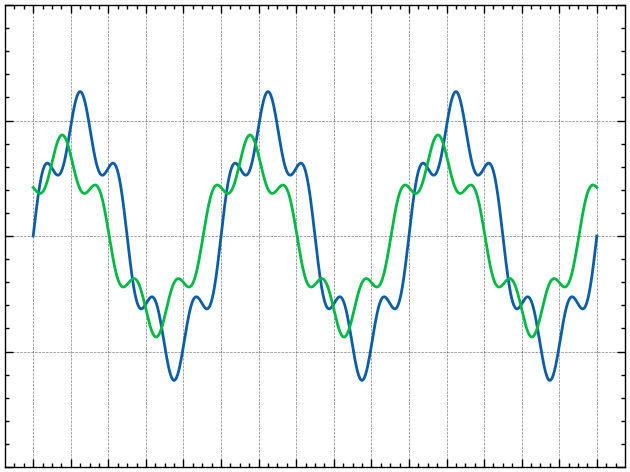
\includegraphics[scale=.6]{err_osci.png}
\caption{Forme de courbe affichée par l'oscilloscope sur les mesures erronées de la seconde expérience}
\label{fig:mes-err}
\end{figure}